\documentclass{article}
\def\pathToRoot{../../}\input{\pathToRoot headers/sharedHeader}

\newtheorem{lemma}{Lemma}
\newtheorem{proposition}{Proposition}
\newtheorem{theorem}{Theorem}
\newtheorem{corollary}{Corollary}
\theoremstyle{definition}
\newtheorem{definition}{Definition}
\newtheorem{example}{Example}

\usetikzlibrary{cd}
\usepackage{subfig}

%\setcounter{equation}{0}
\numberwithin{equation}{section}
\begin{document}
\title{Presheaves, Representables and\\the Yoneda Lemma}
\author{Dominik Wagner}
%\date{June 7, 2017}
\maketitle

\section{Introduction}
In this chapter we prove the following three propositions, which we mentioned earlier but failed to prove directly:
\begin{itemize}
\item If $\cat A$ is cartesian closed and has coproducts, then for all $A,B,C\in\cat A$
  \begin{align*}
    (A\times B)+(A\times C)\iso A\times (B+C);
  \end{align*}
\item Right adjoints are unique up to isomorphisms;
\item For any small category $\cat A$, the category of presheaves $[\cat A^\op,\Set]$ is cartesian closed.
\end{itemize}
Along the way, we prove a very important technical lemma called ``Yoneda lemma''. One of its consequences is that two obects are isomorphic if and only if they ``look the same from all other objects''.

In order to get a first understanding what this is supposed to mean we consider the example of a partially ordered set $(P,\leq)$. Let $p,p'\in P$ be arbitrary. Then we clearly have 
\begin{align*}
  (p\leq p')\iff (\forall q\in P\ldotp q\leq p\rightarrow q\leq p')
\end{align*}
or in other terms
\begin{align}
  \label{eq:pre}
  (p\leq p')\iff {\downarrow}(p)=\{q\in P\mid q\leq p\}\subseteq \{q\in P\mid q\leq p'\}={\downarrow}(p').
\end{align}

How can we lift this to arbitrary categories? We can do so by noting that the two sets correspond to the maps into $p$ and $p'$ respectively. However, since maps between two given objects are not unique in general categories, we have to do a little bit more work. 

Recall the following special functor introduced in chapter 2: 

\begin{definition}[Contravariant Representable Functor]
  Let $\cat A$ be a locally small category and $A\in \cat A$.
 The \demph{contravariant representable functor} of $A$
  \begin{align*}
    H_A=\cat A(-,A)\from \cat A^\op\to \Set
  \end{align*}
  is defined by
  \begin{itemize}
  \item $H_A(B)=\cat A(B,A)$ for objects $B\in\cat A$ and
  \item for maps $f\from B'\to B$:
    \begin{align*}
      H_A(f)=-\of f\from \cat A(B,A)&\to \cat A(B',A)\\
      g &\mapsto g\of f\\\\
      \xymatrix{B' \ar[r]^{f} & B \ar[r]^{g} & A }
    \end{align*}
  \end{itemize}
\end{definition}

Clearly, for each $p$ (in a preorder regarded as a category) ${\downarrow}(p)$ is essentially the same as $H_p$. Furthermore, the inclusions in equation \eqref{eq:pre} correspond to the existence of a natural transformation:
\begin{align*}
  &{\downarrow}(p)=\{q\in P\mid q\leq p\}\subseteq \{q\in P\mid q\leq p'\}={\downarrow}(p')\\
  \iff &\forall q\in P\ldotp q\leq p\rightarrow q\leq p'\\
  \iff &\forall q\in P\ldotp\exists \eta_q\from H_p(q)=P(q,p)\to P(q,p')=H_{p'}(q)\ldotp\top\\
  \iff&\exists \eta\from H_p\to H_q\ldotp\top.
\end{align*}

Thus, the condition in equation \eqref{eq:pre} corresponds to the fact that the following functor is full and faithful:

\begin{definition}[Yoneda Embedding]
  Let $\cat A$ be locally small. The \demph{Yoneda embedding} of $\cat A$ is the functor
  \begin{align*}
    H_-\from \cat A\to[\cat A^\op,\Set]
  \end{align*}
  defined by
  \begin{itemize}
  \item $H_-(A)=H_A$ for objects $A\in\cat A$ and
  \item for maps $f\from A\to A'$, $H_f$ is the natural transformation defined for $B\in \cat A$ by
    \begin{align}
      \label{eq:pre2}
      H_A(B)=\cat A(B,A)&\to H_{A'}(B)=\cat A(B,A')\\
      g&\mapsto  f\of g \nonumber
    \end{align}
  \end{itemize}
  \begin{equation*}
  \xymatrix@C+2pc{
\mathsf{\mathscr{A}^\text{op}} \rtwocell^{H_A}_{H_{A'}}{\;\;\;H_f} & \mathbf{Set}
}
\end{equation*}
\end{definition}
Basically, for preorders \eqref{eq:pre2} constructs a proof from $p\leq p'$ that for all $q\leq p$ also $q\leq p'$ holds.

In what follows we prove that this is indeed an embedding, i.e. full and faithful, in the general case.

\section{Yoneda Lemma}
To do so, we state the following technical lemma due to Yoneda:
\begin{lemma}[Yoneda]
  Let $\cat A$ be locally small. Then
  \begin{align*}
    [\cat A^\op,\Set](H_A,F)\iso F(A)
  \end{align*}
  naturally in $A\in\cat A$ and $F\in [\cat A^\op,\Set]$. That is for each $f\from B\to A$ in $\cat A$ and for each natural transformation $\theta \from F\to F'$ the following commute
  \begin{align*}
    \xymatrix{
    [\cat A^\op,\Set](H_A,F) \ar[r]^{-\of H_f} & [\cat A^\op,\Set](H_B,F) \\
    F(A) \ar[r]^{F(f)} \ar[u]^{\iso}& F(B) \ar[u]_{\iso}
                         } 
  \end{align*}
  \begin{align*}
    \xymatrix{
    [\cat A^\op,\Set](H_A,F) \ar[r]^{\theta\of -} & [\cat A^\op,\Set](H_A,F') \\
    F(A) \ar[r]^{\theta_A} \ar[u]^{\iso} & F'(A) \ar[u]^{\iso}
                             } 
  \end{align*}
\end{lemma}
It is going to help us understand what the arrows $H_A\to H_{A'}$ are (in the presheaf category). More generally, it states that an element of $F(A)$ ``is the same'' as a natural transformation $H_A\to F$.
\begin{proof}
  In order to show the isomorphism in $\Set$, which is supposed to be natural in both $A$ and $F$, we can proceed by:
  \begin{enumerate}
  \item Define a function $(\widehat{-})\from[\cat A^\op,\Set](H_A,F)\to F(A)$.
  \item Define a function $(\widetilde{-})\from F(A)\to[\cat A^\op,\Set](H_A,F)$.
  \item Show that $(\widehat{\widetilde{-}})=1_{F(A)}$.
  \item Show that $(\widetilde{\widehat{-}})=1_{[\cat A^\op,\Set](H_A,F)}$.
  \item Show that $(\widehat{-})$ is natural in $A$.
  \item Show that $(\widehat{-})$ is natural in $F$.
  \end{enumerate}
  It turns out that the definitions of $(\widehat{-})$ and $(\widetilde{-})$ are straightforward as there is only one canonical choice that can possibly be made:
  \begin{enumerate}
  \item Let $\alpha\from H_A\to F$ be arbitrary. In order to define $(\widehat{-})\from[\cat A^\op,\Set](H_A,F)\to F(A)$, we have to come up with an element $\widehat\alpha\in F(A)$. However, $\alpha$ provides us with a function $\alpha_A\from H_A(A)\to F(A)$ in $\Set$. Hence, we only have to come up with an element of $H_A(A)=\cat A(A,A)$ to obtain an element of $F(A)$ and we can simply choose $1_A$. Thus, we define $\widehat\alpha=\alpha_A(1_A)$.
  \item Let $a\in F(A)$. This time, we have to define a natural transformation $\widetilde a\from H_A\to F$, i.e. for each $B\in\cat A$ we have to define a function $\widetilde a_B\from H_A(B)\to F(B)$ in $\Set$ and show that the naturality condition is satisfied.

    In order to define $\tilde a_B$, let $f\in H_A(B)=\cat A(B,A)$ be arbitrary. We have to construct an element of $F(B)$. However, we have a functor $F\from\cat A^\op\to\Set$ and $F(f)\from F(A)\to F(B)$. This is perfect since we already have $a\in F(A)$. Thus, $F(f)(a)\in F(B)$ and we can define 
    \begin{align*}
      \widetilde a_B(f)=F(f)(a).
    \end{align*}

    We still have to check naturality, i.e. that for any $g\from B'\to B$ the following commutes:
    \begin{align*}
    \xymatrix@+2pc{
    H_A(B)=\cat A(B,A) \ar[r]^{H_A(g)=-\of g} \ar[d]^{\widetilde a_B} & H_A(B')=\cat A(B',A) \ar[d]_{\widetilde a_{B'}} \\
    F(B) \ar[r]^{F(g)} & F(B').
                         } 
  \end{align*}
  Since this square is in $\Set$, it suffices to check $(\widetilde a_{B'}\of H_A(g))(f)=(F(g)\of\widetilde a_B)(f)$ for every $f\in H_A(B)=\cat A(B,A)$. Indeed, this holds:
  \begin{align*}
    (\widetilde a_{B'}\of H_A(g))(f)&=(F(f\of g))(a)\\
    &=(F(g)\of F(f))(a)&F \text{ contravariant functor}\\
    &=F(g)(F(f)(a))\\
    &=(F(g)\of\widetilde a_B)(f).
  \end{align*}
\item Let $a\in F(A)$. Clearly, we get $\widehat{\widetilde a}=a$:
  \begin{align*}
    \widehat{\widetilde a}=\widetilde a_A(1_A)=F(1_A)(a)=1_{F(A)}(a)=a.
  \end{align*}
\item[(d)-(f)] The remaining proof obligations are quite straightforward to show and are thus left as an exercise.
  \end{enumerate}
\end{proof}

Now, it is easy to show that $H_-$ is full and faithful by instantiating $F$ with a contravariant representable functor.
\begin{theorem}
  The Yoneda embedding $H_-\from \cat A\to[\cat A^\op,\Set]$ is full and faithful.
\end{theorem}
\begin{proof}
  We have 
  \begin{align*}
    \widehat H_f=(H_f)_A(1_A)=f\of 1_A=f.
  \end{align*}
  Hence,
  \begin{align*}
    \cat A(A,A')&\to[\cat A^\op,\Set](H_A,H_{A'})\\
    f&\mapsto H_f
  \end{align*}
  and
  \begin{align*}
    (\widetilde{-})\from H_{A'}(A)\to[\cat A^\op,\Set](H_A,H_{A'})
  \end{align*}
  are the same function, which are bijective due to the proof of the Yoneda lemma (instantiating $F$ with $H_{A'}$).
\end{proof}

By a previous exercise we know the following:
\begin{lemma}
  \label{lem:ff}
  Let $F\from\cat A\to\cat B$ be a full and faithful functor and $f\from A\to A'$ in $\cat A$.

  Then $f$ is an isomorphism in $\cat A$ if and only if $F(f)$ is an isomorphism in $\cat B$.
\end{lemma}
Thus, we immediately get:
\begin{corollary}[Yoneda Principle]
  Let $\cat A$ be locally small and $A,A'\in\cat A$. Then
  \begin{align*}
    H_A\iso H_{A'} \iff A\iso A'
  \end{align*}
\end{corollary}
Note that the direction from right to left is trivial. Thus, the important consequence of this result is that
\begin{align*}
  H_A(B)=\cat A(B,A)\iso \cat  A(B,A')=H_A'(B) \text{ naturally in } B\in\cat A
\end{align*}
implies $A\iso A'$. Consequently, the following slogan is justified:
\begin{quote}
  \textit{``Two objects are the same if and only if they look the same from all viewpoints.''}
\end{quote}
Abstractly speaking, the Yoneda embedding represents arbitrary locally small categories as presheaf categories, which have much structure. In particular they are cartesian closed.

Note that it is really necessary for the isomorphism to be natural in $B\in\cat A$. This is illustrated by the following example:
\begin{example}
  Consider the following category $\cat A$: 
\begin{align*}
  \xymatrix{
  A \ar@(ul,ur)^{1_A,f} \ar@/^0.3pc/@[][r]^{f_1,f_2} & B \ar@/^0.3pc/@[][l]^{g_1,g_2} \ar@(ul,ur)^{1_B,g}
                                                       } 
  \end{align*}
  i.e. between any pair of object there are two arrows, where the composition of $f_i$ and $g_j$ ($i,j\in\{1,2\}$) is given by
  \begin{align*}
    f_i\of g_j&=g
  \end{align*}
  and the remaining compositions can be chosen arbitrarily.
  
  Obviously,
  \begin{align*}
    \cat A(C,A)\iso\cat A(C,B)
  \end{align*}
  for all $C\in\cat A$ because all homsets contain exactly two elements. However $A\not\iso B$ because by construction neither $g_1$ nor $g_2$ (which are the only maps between $B$ and $A$) have a left inverse.
\end{example}

On the other hand, in special categories it is not even necessary to consider the mappings from \emph{all} other objects. $\Set$ is an extreme such case: Due to the fact that $A\iso\Set[1,A]=H_A(1)$, we have $A\iso A'$ if and only if $H_A(1)\iso H_{A'}(1)$, for all sets $A$ and $A'$.

\section{Consequences of the Yoneda Principle}
Next, we use the insights just gained and we consider (further) consequences of the Yoneda lemma/principle. In particular, we are going to prove the facts mentioned in the introduction.

We start by proving the following ``distributivity''-property:

\begin{proposition}
  \label{prop:dis}
  Let $\cat A$ be cartesian closed such that it has coproducts. Then for all $A,B,C\in\cat A$
  \begin{align*}
    (A\times B)+(A\times C)\iso A\times (B+C).
  \end{align*}
\end{proposition}

For the proof we need the following lemma, which we are also going to use in the proof that presheaf categories are cartesian closed:
\begin{lemma}
  \label{lem:HApres}
  For any locally small category $\cat A$ and $A\in\cat A$, $H_A$ maps all colimits to limits such that $$H_A(\lim_{\to\mathbf I} D)\iso \lim_{\leftarrow\mathbf I}(H_A\of D)$$ for all small categories $\mathbf I$ and diagrams $D\from \mathbf I\to\cat A$.
\end{lemma}
Now the proof of proposition \ref{prop:dis} goes through smoothly:
\begin{proof}[Proof of proposition \ref{prop:dis}]
  We have 
  \begin{align*}
    \cat A(A\times (B+C),X)&\iso\cat A((B+C)\times A,X)\\
                           &\iso\cat A(B+C,X^A)&\cat A\text{ cartesian closed}\\
                           &\iso\cat A(B,X^A)\times \cat A(C,X^A) &\text{by lemma \ref{lem:HApres}}\\
                           &\iso\cat A(A\times B,X)\times \cat A(A\times C,X) &\cat A\text{ cartesian closed}\\
                           &\iso\cat A((A\times B)+(A\times C),X).&\text{by lemma \ref{lem:HApres}}
  \end{align*}
  
  All these isomorphisms are natural in $X\in\cat A$. E.g. the second isomorphism is natural in $X\in\cat A$ because it is induced by a transposition. Hence, we have 
  \begin{align*}
    \cat A^\op(X,A\times (B+C))\iso\cat A^\op(X,(A\times B)+(A\times C))
  \end{align*}
 naturally in $X\in\cat A$ and thus we have $(A\times B)+(A\times C)\iso A\times (B+C)$.
\end{proof}

Another rather easy consequence is that right adjoints are unique:

\begin{proposition}
\label{prop:unique}
  Let $F\from \cat A\to\cat B$ and $G,G'\from\cat B\to\cat A$ such that $F\dashv G$ and $F\dashv G'$. Then $G\iso G'$
\end{proposition}
With the following lemma the proof becomes very nice, indeed:
\begin{lemma}
  \label{lem:comp}
  Let $\cat B$, $\cat C$ and $\cat D$ be categories and $F\from\cat C\to\cat D$ a functor. There is an induced functor
  \begin{align*}
    F\of -\from[\cat B,\cat C]\to [\cat B,\cat D]
  \end{align*}
  defined by composition with $F$. 
Then, $F\of -$ is full and faithful if $F$ itself has these properties.  
\end{lemma}
\begin{proof}[Proof of proposition \ref{prop:unique}]

  By adjointness we get
    \begin{align*}
      H_{G(B)}(A)=\cat A(A,G(B))\iso\cat B(F(A),B)\iso\cat A(A,G'(B))=H_{G'(B)}(A)
    \end{align*}
    naturally in $A\in\cat A$ and $B\in\cat B$. In particular,
    \begin{align*}
      (H_-\of G)(B)=H_{G(B)}\iso H_{G'(B)}=(H_-\of G')(B)
    \end{align*}
    naturally in $B$, i.e. $H_-\of G\iso H_-\of G'$. Due to the lemmas \ref{lem:ff} (``isomorphisms in the image of full and faithful functors are the image of isomorphisms'') and \ref{lem:comp}, as well as the fact that the Yoneda embedding $H_-$ is full and faithful, $G\iso G'$ holds.
  % By adjointness we have 
  % \begin{align*}
  %   \cat B^\op(B,F(A))\iso\cat B(F(A),B)\iso\cat A(A,G(B))\iso\cat B(F'(A),B)\iso\cat B^\op(B,F'(A))
  % \end{align*}
  % naturally in $B\in\cat B$. Hence, by what was stated above we have $F(A)\iso F'(A)$ for all $A\in\cat A$. It can be shown that this isomorphsim is natural in $A$ (why?), hence $F\iso F'$.
\end{proof}
Similarly, it can be shown that left adjoints are unique up to isomorphisms.

\section{Presheaf Category is Cartesian Closed}
In this section we show that for any small category $\cat A$ the presheaf category $[\cat A^\op,\Set]$ is cartesian closed. It is easy to see that it has terminal objects and binary products by defining them ``pointwise''. Showing that exponentials exist is still non-trivial. However the Yoneda lemma provides a straightforward definition of exponentials and in a special case verifying that this is indeed an exponential is simple. In the general case we need a couple of additional lemmas.

Thus, we are left to show that exponentials exists, i.e. that for functors $G,H\in[\cat A^\op,\Set]$, there is a functor $H^G\in[\cat A^\op,\Set]$ such that
\begin{align}
  \label{eq:rem}
  [\cat A^\op,\Set](F,H^G)\iso [\cat A^\op,\Set](F\times G,H)
\end{align}
naturally in $F\in[\cat A^\op,\Set]$.

To define $H^G$ on objects $A\in\cat A$, note that by the Yoneda lemma we have
\begin{align*}
  H^G(A)\iso [\cat A^\op,\Set](H_A,H^G)
\end{align*}
and if $H^G$ is the exponential of $G$ and $H$ we certainly have
\begin{align*}
  [\cat A^\op,\Set](H_A,H^G)\iso [\cat A^\op,\Set](H_A\times G,H).
\end{align*}
Clearly, this set exists and we can thus define
\begin{align*}
  H^G(A)=[\cat A^\op,\Set](H_A\times G,H)
\end{align*}
on objects.
For maps $f\from A\to A'$ we define 
\begin{align*}
  H^G(f)=H^G_f\from [\cat A^\op,\Set](H_{A'}\times G,H)\to[\cat A^\op,\Set](H_A\times G,H)
\end{align*}
 by
$H^G_f(\alpha)\in[\cat A^\op,\Set](H_A\times G,H)$ for $\alpha\in [\cat A^\op,\Set](H_{A'}\times G,H)$, which is a natural transformation and which in turn is defined by
\begin{align*}
  H^G_f(\alpha)_B = (H_g\times 1)\of \alpha_B\from (H_{A}\times G)(B)\to H(B)
\end{align*}
for $B\in\cat A$. This is of course natural.

Therefore, we are left to verify that \eqref{eq:rem} holds and that it is natural in $F\in[\cat A^\op,\Set]$.
In order to understand the proof better let us first consider the special case where $F=H_A$ is a covariant representable functor for some $A\in\cat A$. Then, we immediately have
\begin{align*}
  [\cat A^\op,\Set](H_A,H^G)&\iso H^G(A)&\text{Yoneda lemma}\\
  &=[\cat A^\op,\Set](H_A\times G,H).&\text{definition of }H^G
\end{align*}

Unfortunately, we have to show that this natural in \emph{all} $F\in[\cat A^\op,\Set]$, not just covariant representable functors, and not every functor is isomorphic to some $H_A$. However, it turns out that each presheaf is a \emph{colimit} of representable functors:

\begin{lemma}
  \label{lem:lim}
  For any small category $\cat A$, any functor $F\from\cat A^\op\to\Set$ is a colimit of representable functors,
  \begin{align*}
    \lim_{\to I\in\mathbf I} H_{\pi(I)}\iso F
  \end{align*}
  for some small category $\mathbf I$ and functor $\pi\from \mathbf I\to \cat A$.
\end{lemma}
\begin{proof}
  First of all, we have to define the shape of the limit, i.e. a small category $\mathbf I$. We take the \emph{category of elements} of $F$, $\int_{\cat A}F$ with
  \begin{itemize}
  \item objects being pairs $(a,A)$ such that $A\in\cat A$ and $a\in F(A)$;
  \item arrows $f\from(a,A)\to(b,B)$ being arrows $f\from A\to B$ in $\cat A$ such that $F(f)(b)=a$.
  \end{itemize}

\begin{figure}
  \subfloat[A category $\cat A$ with two objects and one map.]
  {%
    \begin{tikzpicture}
      \draw[draw=white] (-1.2,0) ellipse (0.75cm and 1.3cm);
      \node[] at (-1.2, 0)     (A) {$A$};
      \node[] at (1.2, 0)    (B) {$B$};
      \path[draw,->] (A) -- (B);
    \end{tikzpicture}
  }\hfill
  \subfloat[Its image under a presheaf $F$, where $F(A)=\{a_1,a_2,a_3\}$ and $F(B)=\{b_1,b_2\}$, as well as $b_1\mapsto a_1$ and $b_2\mapsto a_3$.]
  {
    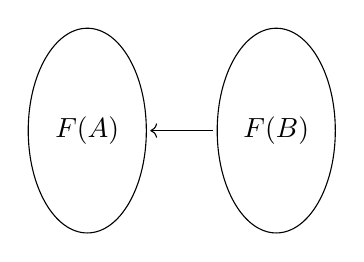
\begin{tikzpicture}
      \draw (-1.2,0) ellipse (0.75cm and 1.3cm);
      \draw (1.2,0) ellipse (0.75cm and 1.3cm);
      \node[] at (-1.2, 0)   (fa) {$F(A)$};
      \node[] at (1.2, 0)   (fb) {$F(B)$};
      \path[draw,<-] (-0.4,0) -- (0.4,0);
    \end{tikzpicture}
  }\hfill
\subfloat[The corresponding category of elements $\int_{\cat A}F$.]
  {
    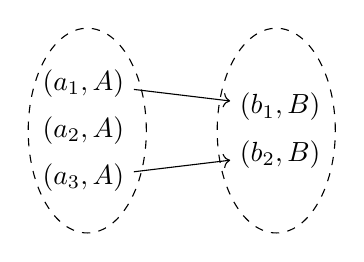
\begin{tikzpicture}
      \draw[dashed] (-1.2,0) ellipse (0.75cm and 1.3cm);
      \draw[dashed] (1.2,0) ellipse (0.75cm and 1.3cm);
      \node[] at (-1.25, 0.6)   (aA1) {$(a_1,A)$};
      \node[] at (-1.25, 0)     (aA2) {$(a_2,A)$};
      \node[] at (-1.25, -0.6)  (aA3) {$(a_3,A)$};
      \node[] at (1.25, 0.3)    (bB1) {$(b_1,B)$};
      \node[] at (1.25, -0.3)   (bB2) {$(b_2,B)$};
      \path[draw,->] (aA1) -- (bB1);
      %\path[draw,->] (aA2) -- (bB1);
      \path[draw,->] (aA3) -- (bB2);
    \end{tikzpicture}
  }
  
  \caption{\label{fig:ex}Visualization of a category and its corresponding category of elements (identities are omitted).}
\end{figure}

  and identities and composites are defined in the natural way. Figure \ref{fig:ex} contains a visualization of a category and its corresponding category of elements. Clearly, $\int_{\cat A}F$ is small since $\cat A$ is small.

  Next, we have to define a diagram $\int_{\cat A}F\to[\cat A^\op,\Set]$ such that $F$ is the corresponding limit. We simply take $H_-\of\pi$ where $\pi\from \int_{\cat A}F\to\cat A$ is the projection on $\cat A$ defined by 
  \begin{itemize}
  \item $\pi(a,A)=A$ on objects and
  \item $\pi(f)=f$ on arrows in $\cat A$ .
  \end{itemize}

  Now, we have to verify that $F$ is indeed the limit of $H_-\of\pi$ under $\int_{\cat A}F$, i.e. we have to specify a cocone
  \begin{align*}
    (H_{\pi(a,A)}\to F)_{(a,A)\in \int_{\cat A}F}
  \end{align*}
  and show that it is universal amongst all cocones.

  To define $H_{\pi(a,A)}=H_A\to F$ for any $(a,A)\in \int_{\cat A}F$ we recall that $[\cat A^\op,\Set](H_A,F)\iso F(A)$, where the isomorphism from the right to the left is given by $(\widetilde -)$ (as defined in the proof of the Yoneda lemma). Thus, we define the $(a,A)$-component of the cocone to be $\widetilde a$. For this to be a cocone we still have to verify that for each $f\from (b,B)\to (a,A)$ (i.e. $f\from B\to A$ such that $F(f)(a)=b$)
  \begin{align*}
    \xymatrix@+1.5pc{
      H_{\pi(b,B)}=H_B \ar[r]^{\widetilde b} \ar[d]_{H_{\pi(f)}=H_f} & F \\
      H_{\pi(a,A)}=H_A \ar[ru]_{\widetilde a} & 
                         } 
  \end{align*}
  commutes. However, by the naturality statement for $A\in\cat A$ in the Yondea lemma we have that 
  \begin{align*}
    \xymatrix@+1pc{
    [\cat A^\op,\Set](H_A,F) \ar[r]^{-\of H_f} & [\cat A^\op,\Set](H_B,F) \\
    F(A) \ar[r]^{F(f)} \ar[u]^{(\widetilde-)}& F(B) \ar[u]_{(\widetilde -)}
                         } 
  \end{align*}
  commutes. In particular for any $a\in F(A)$ we have
  \begin{align*}
    \widetilde a\of H_f=\widetilde{F(f)(a)}=\widetilde b
  \end{align*}
  by definition of arrows in $\int_{\cat A}F$.

  Thus, we have shown that this indeed constitues a cocone. Similarly, it can be shown that this cocone is universal, i.e. that $F$ is the limit of $H_-\of\pi$ under $\int_{\cat A}F$.
\end{proof}

Now, we are almost in a position where we can prove that presheaf categories are cartesian closed. All we need is the following lemma (the proof of which is left as an exercise) which states that we can ``pull limits out of products'':
\begin{lemma}
  \label{lem:pull}
  Let $F\from \cat A\to\Set$ be a presheaf. The functor $-\times F\from [\cat A^\op,\Set]\to[\cat A^\op,\Set]$ preserves colomits. That is:
  \begin{align*}
    \lim_{\to \mathbf I} (D\times F)\iso (\lim_{\to \mathbf I} D)\times F
  \end{align*}
  for any small category $\mathbf I$ and functor $D\from\mathbf I\to [\cat A^\op,\Set]$.
\end{lemma}
Finally, we can prove
\begin{proposition}
  For any small category $\cat A$, the category of presheaves $[\cat A^\op,\Set]$ is cartesian closed.
\end{proposition}
\begin{proof}
  It is easy to prove that $[\cat A^\op,\Set]$ has terminal objects and binary products (by defining them ``pointwise'').

  With the previous definitions we are left to verify that 
  \begin{align*}
    [\cat A^\op,\Set](F,H^G)\iso [\cat A^\op,\Set](F\times G,H)
  \end{align*}
  naturally in $F\in[\cat A^\op,\Set]$. Using lemma \ref{lem:lim} we have
  \begin{align*}
    F\iso\lim_{\to I\in\mathbf I} H_{\pi(I)}.
  \end{align*}
Hence, we conclude:
  \begin{align*}
    [\cat A^\op,\Set](F,H^G)&\iso [\cat A^\op,\Set](\lim_{\to I\in\mathbf I} H_{\pi(I)},H^G)&\\
                            &\iso \lim_{\leftarrow I\in\mathbf I} [\cat A^\op,\Set](H_{\pi(I)},H^G)&\text{by lemma \ref{lem:HApres}}\\
                            &\iso \lim_{\leftarrow I\in\mathbf I} H^G(\pi(I))&\text{by the Yoneda lemma}\\
                            &\iso \lim_{\leftarrow I\in\mathbf I} [\cat A^\op,\Set](H_{\pi(I)}\times G,H)&\text{by definition of } H^G\\
                            &\iso [\cat A^\op,\Set](\lim_{\to I\in\mathbf I}(H_{\pi(I)}\times G),H)&\text{by lemma \ref{lem:HApres}}\\
                            &\iso [\cat A^\op,\Set](\lim_{\to I\in\mathbf I}(H_{\pi(I)})\times G,H)&\text{by lemma \ref{lem:pull}}\\
                            &\iso[\cat A^\op,\Set](F\times G,H).
  \end{align*}
  All the isomorphisms are natural in $F$. Thus $H^G$ is indeed the exponential of $G$ and $H$.
\end{proof}

\section{Conclusion}
In this chapter we studied the Yoneda lemma and some of its consequences. It states that for any presheaf $F$ and object $A$, $F(A)$ is isomorphic to the set of presheaves $H_A\to F$ (and that the isomorphism is natural in $F$ and $A$). A consequence is that any locally small category can be embedded in a presheaf category, which has much more structure. Informally, two objects are isomorphic if and only if they look the same from all other objects.

As applications, we proved a distributivity-property in cartesian closed categories that have copro\-ducts and we showed that right adjoints are unique up to isomorphisms.

Finally, the proof that presheaf categories are cartesian closed elaborated on the statement above that we gain structure by means of the Yoneda embedding.

\end{document}

% vim mode line:
% vim: ts=2 sts=2 sw=2 expandtab

%%% Local Variables:
%%% mode: latex
%%% TeX-master: t
%%% End:
